\documentclass[english,a4paper,11pt]{report}
\usepackage[utf8]{inputenc}
\usepackage[T1]{fontenc}
\PassOptionsToPackage{english}{babel}
\usepackage{graphicx}
\usepackage{fullpage}
\usepackage{eso-pic}
\usepackage{cite}
\usepackage{wrapfig}
\usepackage{url}
\usepackage[english]{babel}
\usepackage{fancyhdr}
\usepackage{hyperref}
\usepackage[lastpage,user]{zref}
\cfoot{\thepage\ of \zpageref{LastPage}}
\pagestyle{fancy}
\usepackage[headsep=1cm,headheight=61pt,footskip=3cm]{geometry}


\newcommand{\HRule}{\rule{\linewidth}{0.5mm}}
 \newcommand{\ts}{\textsuperscript}
\newcommand{\blap}[1]{\vbox to 0pt{#1\vss}}
\newcommand\AtUpperLeftCorner[3]{%
  \put(\LenToUnit{#1},\LenToUnit{\dimexpr\paperheight-#2}){\blap{#3}}%
}
\newcommand\AtUpperRightCorner[3]{%
  \put(\LenToUnit{\dimexpr\paperwidth-#1},\LenToUnit{\dimexpr\paperheight-#2}){\blap{\llap{#3}}}%
}
\newcommand\AtLowerRightCorner[3]{%
  \put(\LenToUnit{\dimexpr\paperwidth-#1},\LenToUnit{#2}){#3}%
}
 
\title{\LARGE{Internship report pattern recognition UNISA Italy}}
\author{\textsc{Breton-Belz} Emmanuel - 2\ts{nd} Year Internship}
\date{\today}
\makeatletter

\renewcommand{\headrulewidth}{1pt}
\fancyhead[C]{\@author} 
\fancyhead[L]{\leftmark}
\fancyhead[R]{
\includegraphics[width=2cm]{images_not_compressed/unisaLogo.jpg}}
\fancyhead[L]{{
\includegraphics[width=2cm]{images_not_compressed/ensiLogo.jpg}}}
\addto\captionsenglish{
  \renewcommand{\contentsname}
    {Table of contents}
}
\renewcommand{\footrulewidth}{1pt}
\fancyfoot[R]{\leftmark}
		 
\begin{document}
	\setcounter{tocdepth}{4}
	\begin{titlepage}
	    \AddToShipoutPicture{%
	      \AtUpperLeftCorner{1.5cm}{1cm}{
\includegraphics[width=4cm]{images_not_compressed/unisaLogo.jpg}}
	      \AtUpperRightCorner{1.5cm}{1cm}{
\includegraphics[width=6.5cm]{images_not_compressed/ensiLogo.jpg}}
	      \AtLowerRightCorner{8cm}{3.5cm}{\parbox{7cm}{ENSICAEN \\
	        6, boulevard Maréchal Juin 
	        \\CS  45 053 – F- 14050 Caen Cedex 4\\
	        Tél. +33 (0)2 31 45 27 50\\
	        Fax +33 (0)2 31 45 27 60}} 
	    }
	 
	\begin{center}
	        \vspace*{10cm}
	        \textsc{\@title}
	        \HRule
	        \vspace*{0.5cm}
	        \large{\@author} 
	 \end{center}
 
    \vspace*{5cm}
    \begin{center}
      \makebox[\textwidth]{
\includegraphics[width=\paperwidth]{images_not_compressed/uneGrandeEcole.png}}
    \end{center}
	
	\end{titlepage}
	\ClearShipoutPicture
	
	\chapter*{Thanks}
\par I would like to thank Mario Vento for hosting me in the labs, giving me the opportunity to see conferences of foreign computer scientists and following me during the internship.	
\par I thank Pierluigi Ritrovato who gave me my subjects, guided me to my targets and answered my questions.
\par I Thank Hugo Descoubes too, who helped me during the first part of my internship. 
\par Finally, I want to thank Allessia who contacted me for the papers and gave me good advices on the matching system and the international relation departement of ENSICAEN which prepared all the documents for ERASMUS facilities.
	
	
	
	\tableofcontents
	\newpage
	
	\setcounter{page}{1}
	
	\chapter{Introduction}

\par During the second year of engineering school at ENSICAEN we have 3 month internship that I decided to do in the MIVIA Lab of Salerno's university in italy. They are specialised in image synthesis which is my major course, moreover I am interested in a double diploma in this unversity which gives me the opportunity to see the place and teachers, learn the italian and make some contacts.
\par My internship subject has been splited in two. First a study on the Motorola HC1 helmet used for exemple in military domain. The aim was to see if we could make the helmet compile Linux for helmet. Then developpe an application capable of recognise patterns in an image and store the position, the number of patterns found and the type of each pattern. So as to determine the name of a global structure which the patterns are composants.
\par In this report I will present the laboratory and the place of the internship, the study of the hardware for the helmet and the software (OpenCV mainly) for the application. What exists and where my projects are situated in their environnements. After that I explain what I tried to slove the problems and what are the results.
	\chapter[MIVIA Lab]{The MIVIA Laboratory}

\begin{wrapfigure}[2]{l}{2cm}
	\vspace{-7mm}
	
\includegraphics[width=2cm]{images_not_compressed/MIVIALogo.jpg}
	\end{wrapfigure}
 for Macchine Intelligenti per il riconoscimento di Video, Immagini e Media which means intelligent machines for video, images and media recognition. The laboratory is located in Fisciano, Campania, Italy. 
 
 \par As its name suggest besides theaching computer science, the doctors of the lab work on pattern recognition, classification, media analysis and many parallele subjects like autonomus drones and robot vision.
	\chapter{Evaluation of the need}

\section{Helmet HC1 needs}
\begin{wrapfigure}[13]{r}{6cm}
 \begin{center}
	 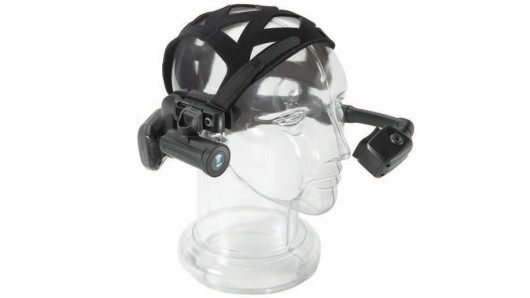
\includegraphics[width=6cm]{images_not_compressed/motorola_hc1.jpg}
		\caption{Picture of the HC1 helmet with the camera plugged}
		\label{hc1}
	 \end{center}
 \end{wrapfigure}

 \par The HC1 Helmet from Motorola is a professional use helmet dedicated to wide or site conditions. It costs around 3000\$ with the camera. It is used to show images in augmented reality in the little screen in front of the left eye. Full voice commanded, it uses an embedded version of windows which was a real problem. You can look at the figure~\ref{hc1} to have an idea of what it looks like.
 
 \par Despite the fact that the Helmet is thought to add functionnalities, a client of the MIVIA Lab asked them if it was possible to install Linux or Android on the helmet. Even if they loose the voice command system and the drivers to run the camera etc. They asked me to try, at least, to do it.

\section{The software needs}
 \par At work, when people have to make maintenance of the material, they encounter a problem with the density of the maintenance manuals which can make around 700 pages. We try to ease the maintenance by recreating manuals that focuses on the material that the technician is looking at. To obtain this result, we have to analyze the images of the camera and extract the type of material. That is what the laboratory asked me to do.
 \par This solution can apply to a lot of other objects to find monuments and extract their description for exemple. To do that I had to use OpenCV pattern detection via SIFT points matching.  
	
	\chapter[Studies]{Study of the existing}
Once again this part will be splitted in 2 because the subjects are totally differents. I am going to talk first about the helmet, that required 1 month of test and studies. I will explain the procedures in the next chapter. 
	
	\section{Helmet study}	
	\subsection{Helmet itself}
	\par I began my study by acquire some knowledges about the helmet itself. It has been release in the end of 2013, build for harsh condition, its price makes it unaccessible for the public. The army and building companies sow a good opportunity in this technologie to ease the work by bringing communication into the field.
	\par The helmet is equiped with a batterie, Wi-Fi and blutooth connections, a camera and it can be wear under the work helmet. Everything is voice commanded and very responsive thanks to Motorola's work. Windows CE 6.0 is used on the last release of the helmet image. It is good for the next section to understand that the booting system and the update system of windows CE are related. That means that you can change the file system for an update but it is windows itself that validate and copy the files on the intern memory from the SD card.
	\subsection{Embedded systems}
	\par I learned a lot about embbeded system, mainly on the boards and all the materials related to it. In our case, the materials inside the helmet are not know and not published on the Internet. Pierluigi contacted the company that brought us the helmet but they couldn't tell us which board was used in the helmet. I must have guessed which TI technology it was because the datasheet reference a TI OMAP 3 microprocessor. 
	\par That is mainly why I put my effort on the "ISEE – IGEP COM MODULE" built in with a TI OMAP 3 processor. It was at the top of the art when the helmet released and the smallest board with this processor. It corresponds well with the size of the hardware slot. In any case, if the linux kernel is compatible with the processor a cross compiled file system should boot and at least it should show an image on the screen.
	
	\subsection{Cross-compilation}
	\subsubsection{Description}
	\par The cross-compilation is compilation for a different achitecture than the architecture that makes the computations. In the figure~\ref{cross} you can see that the source code can be compiled for different architectures. The aim here was to compile a Linux kernel compatible with TI OMAP 3 processors from an Intel x86 machine.
	\begin{figure}[h]
		\begin{center}
			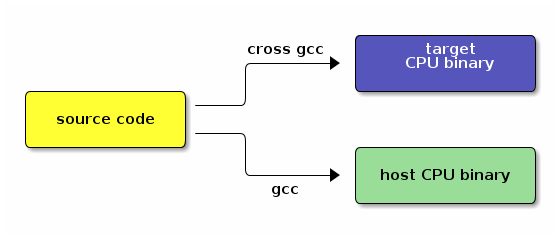
\includegraphics[scale=0.5]{images_not_compressed/cross-compile.png}
			\label{cross}
			\caption{Cross compilation and compilation difference}
		\end{center}
	\end{figure}

	\subsubsection{Process}
	\par The cross tool chain is capable of compile a Linux kernel for a lot of achitectures. Of course it requires a long time to compile the toolchain and then cross compile the kernel to get the binaries but it is cost effective. The time necessere to compile the toolchain and the kernel on the TI OMAP 3 would be longer.
	
	\subsubsection{Toolchain}
	
	\par A toolchain is a set of distinct software development tools that are linked (or chained) together by specific stages such as GCC, binutils and glibc (a portion of the GNU Toolchain)\cite{Toolchain}.
	\par A toolchain requires binutils such as assembler and linker, that produces the binaries. Also compilers for deferent languages like C, C++, Java etc, that transforms any language into another. A C library to gain access to kernel calls and a debugger that can be used or not during the compilation. We can see well on the diagram \ref{compchain} from (avrfreaks.net's forum)  where each composant is located :
	\begin{figure}[ht]
		\begin{center}
			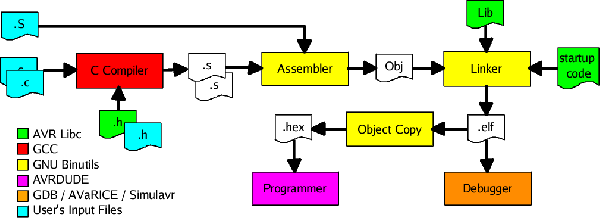
\includegraphics[scale=0.5]{images_not_compressed/compchain.png}
			\label{compchain}
			\caption{Cross compilation and compilation difference}
		\end{center}
	\end{figure}

		
	\section{Pattern recognition study}
	\subsection{OpenCV}
	
		\begin{wrapfigure}[4]{l}{2cm}
	\vspace{-7mm}
	
\includegraphics[width=2cm]{images_not_compressed/opencv_logo.png}
	\end{wrapfigure}
	\par OpenCV is an image analysis and synthesis library that brings all the necessary for video and photo analysis. Introduced in 2000, it is now used a lot in the fields that require image analysis.
 It is built around a modular system that allows users to install the library depending on their needs.
 Except the non free module, the library is licensed BSD which means that we can reuse and modify all the components freely.
 In this document I will talk more about precise modules of OpenCV as a base and features2d modules.
	
	\subsection{Existing code}
	
	\par To get some examples of code and see how it works I simply looked at the OpenCV tutorials that are available on the internet. For example check~\hyperlink{opencv}{it in the annexe section}. It brings a simple way to extract a pattern and make the homography to draw the corners with lign OpenCV function.
	
	\subsubsection{Key points}
	\par SIFT points are points of interest in the image. They give the position of an area where all the pixels have approximately the same properties. Using the Laplacian of Gaussian of the image, maxima and minima which correspond to these areas can be extracted.
	\par The biggest advantage of these points is the invariance in transformation like rotation, scaling and translation. Pattern detection algorithm based on this point is insensitive in term of scale and rotation. That is mainly why it has been chosen for this application.
	\par As a result, by the time that the resolution of the pattern is over an acceptable threshold. We can move and rotate the object without altering the detection.
	
	\subsubsection[Descriptor]{SIFT Descriptor}
	\par The descriptors are computed from the key points. The descriptors associated with the SIFT key points are locally oriented histograms around a SIFT key point \cite{AM}:
	
	\begin{itemize}
			\item We divide space around each key point (x, y) in N\ts{2} squares of 4 by 4 \item We compute the gradient \begin{math}G_{x}(a,b,\sigma)\end{math}, \begin{math}G_{y}(a,b,\sigma)\end{math} for the 4 by 4 by N\ts{2} points (a, b)

		\item For each 4 by 4 square, we compute a histogram of the orientations in 8 directions, multiplying by: (1) the module of the gradient (2) the inverse of the distance to the key point (x, y).
 \item To be invariant in rotation: the local orientation of the key point \begin{math} \theta(x,y) \end{math} is used as the origin (null orientation) of the histograms.		
	\end{itemize}
	
	
	\subsubsection{Homography}
	\par  Just to give a simplified idea, the familiar Cartesian plane is composed by a set of points which have a one-to-one correlation to pairs of real numbers, i.e. X-Y on the two axis\cite{Homography}.
	\par In our case, the points are the key points extracted. By extracting the homography matrix, we can transform the corners of our image to 4 other points representing the position of the object on the scene\cite{TutoHomography}.
	
	\begin{wrapfigure}[12]{r}{10cm}
			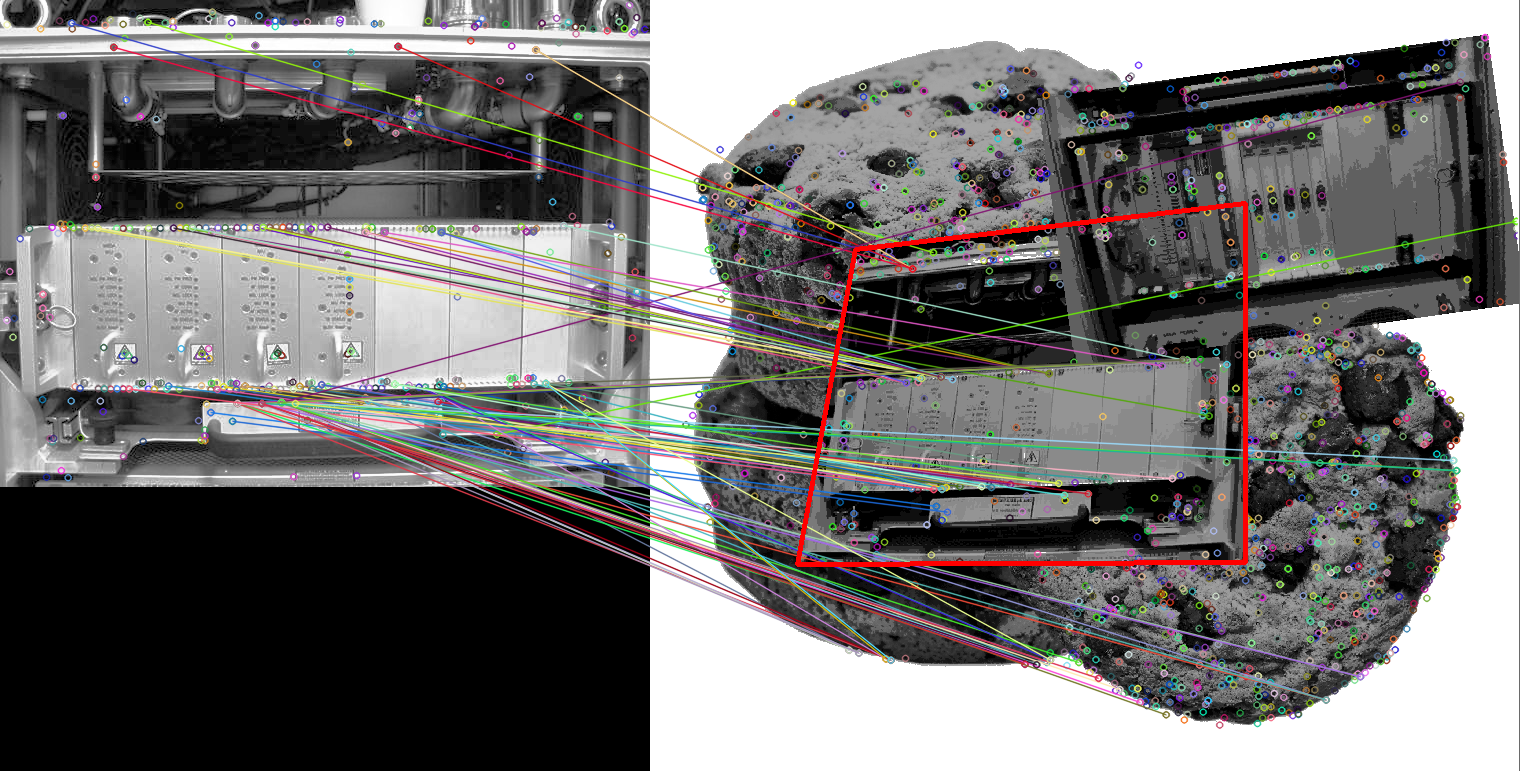
\includegraphics[width=10cm]{images_not_compressed/showHomography.png}
			\caption{Homography with a corner hidden with openCV}
	\end{wrapfigure}
	\par On the image behind we can see that the homography doesn't depend on the corners. All the key points can be a base to analyze the transformation. And using the perspective transform of OpenCV that multiplies the corners by the homography matrix. We obtain the position of the corners on the captured image.


	Once again this part will be splitted in 2 because the subjects are totally differents. I am going to talk first about the helmet, that required 1 month of test and studies. I will explain the procedures in the next chapter. 
	
	\section{Helmet study}	
	\subsection{Helmet itself}
	\par I began my study by acquire some knowledges about the helmet itself. It has been release in the end of 2013, build for harsh condition, its price makes it unaccessible for the public. The army and building companies sow a good opportunity in this technologie to ease the work by bringing communication into the field.
	\par The helmet is equiped with a batterie, Wi-Fi and blutooth connections, a camera and it can be wear under the work helmet. Everything is voice commanded and very responsive thanks to Motorola's work. Windows CE 6.0 is used on the last release of the helmet image. It is good for the next section to understand that the booting system and the update system of windows CE are related. That means that you can change the file system for an update but it is windows itself that validate and copy the files on the intern memory from the SD card.
	\subsection{Embedded systems}
	\par I learned a lot about embbeded system, mainly on the boards and all the materials related to it. In our case, the materials inside the helmet are not know and not published on the Internet. Pierluigi contacted the company that brought us the helmet but they couldn't tell us which board was used in the helmet. I must have guessed which TI technology it was because the datasheet reference a TI OMAP 3 microprocessor. 
	\par That is mainly why I put my effort on the "ISEE – IGEP COM MODULE" built in with a TI OMAP 3 processor. It was at the top of the art when the helmet released and the smallest board with this processor. It corresponds well with the size of the hardware slot. In any case, if the linux kernel is compatible with the processor a cross compiled file system should boot and at least it should show an image on the screen.
	
	\subsection{Cross-compilation}
	\subsubsection{Description}
	\par The cross-compilation is compilation for a different achitecture than the architecture that makes the computations. In the figure~\ref{cross} you can see that the source code can be compiled for different architectures. The aim here was to compile a Linux kernel compatible with TI OMAP 3 processors from an Intel x86 machine.
	\begin{figure}[h]
		\begin{center}
			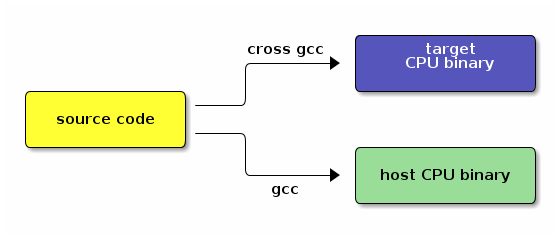
\includegraphics[scale=0.5]{images_not_compressed/cross-compile.png}
			\label{cross}
			\caption{Cross compilation and compilation difference}
		\end{center}
	\end{figure}

	\subsubsection{Process}
	\par The cross tool chain is capable of compile a Linux kernel for a lot of achitectures. Of course it requires a long time to compile the toolchain and then cross compile the kernel to get the binaries but it is cost effective. The time necessere to compile the toolchain and the kernel on the TI OMAP 3 would be longer.
	
	\subsubsection{Toolchain}
	
	\par A toolchain is a set of distinct software development tools that are linked (or chained) together by specific stages such as GCC, binutils and glibc (a portion of the GNU Toolchain)\cite{Toolchain}.
	\par A toolchain requires binutils such as assembler and linker, that produces the binaries. Also compilers for deferent languages like C, C++, Java etc, that transforms any language into another. A C library to gain access to kernel calls and a debugger that can be used or not during the compilation. We can see well on the diagram \ref{compchain} from (avrfreaks.net's forum)  where each composant is located :
	\begin{figure}[ht]
		\begin{center}
			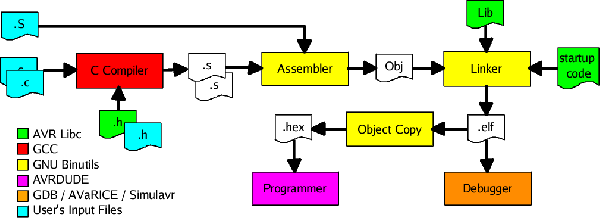
\includegraphics[scale=0.5]{images_not_compressed/compchain.png}
			\label{compchain}
			\caption{Cross compilation and compilation difference}
		\end{center}
	\end{figure}

	
	\section{Pattern recognition study}
	\subsection{OpenCV}
	\subsection{Existing code}

	\chapter{Achievements}
	\chapter{conclusion}

	\clearpage

\bibliography{/home/manu/workspace/Scanner/Report/biblio_internship}{}
	\bibliographystyle{plain}


	\listoffigures
	
	\chapter*{Summary}

	
	
\end{document}